% !TEX TS-program = pdflatex
% !TEX encoding = UTF-8 Unicode

% This is a simple template for a LaTeX document using the "article" class.
% See "book", "report", "letter" for other types of document.

\documentclass[11pt]{article} % use larger type; default would be 10pt

\usepackage[utf8]{inputenc} % set input encoding (not needed with XeLaTeX)

%%% Examples of Article customizations
% These packages are optional, depending whether you want the features they provide.
% See the LaTeX Companion or other references for full information.

%%% PAGE DIMENSIONS
\usepackage{geometry} % to change the page dimensions
\usepackage{graphicx}
\geometry{a4paper} % or letterpaper (US) or a5paper or....
% \geometry{margin=2in} % for example, change the margins to 2 inches all round
% \geometry{landscape} % set up the page for landscape
%   read geometry.pdf for detailed page layout information

\usepackage{graphicx} % support the \includegraphics command and options

% \usepackage[parfill]{parskip} % Activate to begin paragraphs with an empty line rather than an indent

%%% PACKAGES
\usepackage{booktabs} % for much better looking tables
\usepackage{array} % for better arrays (eg matrices) in maths
\usepackage{paralist} % very flexible & customisable lists (eg. enumerate/itemize, etc.)
\usepackage{verbatim} % adds environment for commenting out blocks of text & for better verbatim
\usepackage{subfig} % make it possible to include more than one captioned figure/table in a single float
% These packages are all incorporated in the memoir class to one degree or another...

%%% HEADERS & FOOTERS
\usepackage{fancyhdr} % This should be set AFTER setting up the page geometry
\pagestyle{fancy} % options: empty , plain , fancy
%\setlength{\headheight}{-25pt}
\renewcommand{\headrulewidth}{0pt} % customise the layout...
\lhead{}\chead{}\rhead{}
\lfoot{}\cfoot{\thepage}\rfoot{}

%%% SECTION TITLE APPEARANCE
\usepackage{sectsty}
\allsectionsfont{\sffamily\mdseries\upshape} % (See the fntguide.pdf for font help)
% (This matches ConTeXt defaults)

%%% ToC (table of contents) APPEARANCE
\usepackage[nottoc,notlof,notlot]{tocbibind} % Put the bibliography in the ToC
\usepackage[titles,subfigure]{tocloft} % Alter the style of the Table of Contents
\renewcommand{\cftsecfont}{\rmfamily\mdseries\upshape}
\renewcommand{\cftsecpagefont}{\rmfamily\mdseries\upshape} % No bold!

%%% END Article customizations

%%% The "real" document content comes below...

\title{Homework 4}
\author{Maksim Levental}
%\date{} % Activate to display a given date or no date (if empty),
         % otherwise the current date is printed 

\usepackage{listings}
\usepackage{color}

\definecolor{dkgreen}{rgb}{0,0.6,0}
\definecolor{gray}{rgb}{0.5,0.5,0.5}
\definecolor{mauve}{rgb}{0.58,0,0.82}

\lstset{frame=tb,
  language=C++,
  aboveskip=3mm,
  belowskip=3mm,
  showstringspaces=false,
  columns=flexible,
  basicstyle={\small\ttfamily},
  numbers=left,
  numberstyle=\tiny\color{gray},
  keywordstyle=\color{blue},
  commentstyle=\color{dkgreen},
  stringstyle=\color{mauve},
  breaklines=false,
  breakatwhitespace=false,
  tabsize=3,
  frame=0
}

\begin{document}
\maketitle

\section*{Problem 1}
\subsection*{a}
The size of the virtual address is 2\textsuperscript{32} addresses which equals 4294967296 virtually accessible byte addresses. 
\subsection*{b}
4294967296/2048 = 2097152 pages
\subsection*{c}
512*1024*1024/2*1024 = 512*512 = 262144 page frames.
\subsection*{d}
2\textsuperscript{11} = 2048 hence 11 bits.
\subsection*{e}
32-11 = 21 so 21 bits for the page number.
\subsection*{f}
\subsubsection*{i}
2097152 pages * 16 bytes = 32 MB.
\subsubsection*{ii}
262144 page frames * 16 bytes = .25 MB.
\subsubsection*{iii}
We will first divide the virtual address into 4 parts (segment table, page table dir, page table, offset). If we assume Segmentation with Paging the offset gets 11 bits, the page tables get 7 bits, the page directories get 7 bits, and the segment table gets 7 bits. So each level can index 2\textsuperscript{7} sublevels, which is 128. So there are 128 entries in the Segment Table, then 128 page directories each with 128 entries, and finally 128 page tables per page directory each with 128 page table entries. This is 128+128*128+128*128*128 = 2113664 entries, which times 16 bytes is 32.25MB. Finally at the third level we can store all of the stack in one page table (because the stack needs only 120 entries < 128) and all of text+data in 2 tables (because text+data need 230 entries > 128). These page tables should be pointed to from the top and bottom of whichever page directory they're pointed to from. All other page directory and page table entries should point to null. The diagram below shows a schematic. The final level of page tables point to page frames in physical memory.

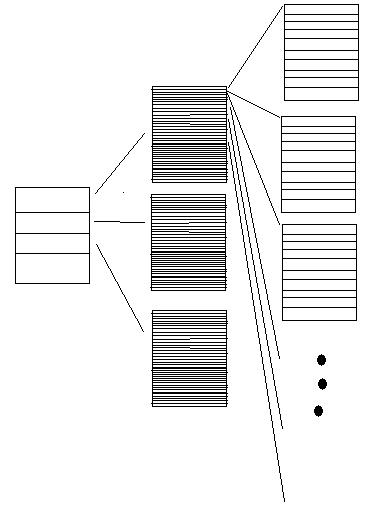
\includegraphics[scale=2]{Untitled.png}



\section*{Problem 2}
\begin{lstlisting}
int x = 5;
int main()
{
	int pid = fork();
	if (pid == 0)
	{
		printf("I'm the child\n");
		x = 10;
		execvp(...);
		return -1;
	}
	else if (pid > 0)
	{
		printf("I'm the parent\n");
	}
return 0;
}
\end{lstlisting}

Line 4 causes a copy of the stack segment, because fork() is a function call. Line 8 is a write by the child so it causes a copy of the data segment to be made (because x is a global variable and so is in the data segment). Line 9 calls execvp so it causes a copy of the text segment to be made.

\section*{Problem 3}

\subsection*{i}
The virtual address is divided into 4 parts. Diagram:

 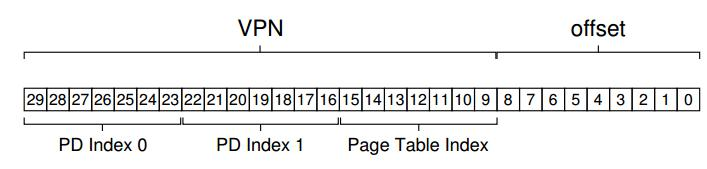
\includegraphics{untitled1.JPG}
\subsection*{ii}

PD Index 0 indexes into the first Page Directory table, PD Index 1 indexes into the second Page Directory table, Page Table index indexes in the page table (selecting the page), and then finally offset indexes into the page.

\subsection*{iii}

PD Index 0 is added to the base address stored in a system register in order to find the correct entry in the first Page directory. This entry then has a link to the base address of the second Page directory. To this base address is added PD Index 1 to find the correct entry for the Page Table. This entry contains a link to the Page Table to which the Page Table index is added to find the Page Table Entry. This entry then points to the correct page frame. The offest is then added to the base address of page frame in memory to get the correct memory address.

\section*{Problem 4}
\subsection*{a}
The block will be put into the first large enough spot: it will be put at address 31844.
\subsection*{b}
The block will be put into the gap with the least amount of internal fragmentation: it will be put at address 44680.
\subsection*{c}
The block will be put into the largest block: it will be put at address 1096.
\subsection*{d}
The block will be put into the first fit after the current pointer (including checking the current pointer). Since it doesn't fit into the current pointed to gap, it gets put into the next one that it fits into, which is the one at 1096.
\section*{Problem 5}
\subsection*{Fixed Partitioning with Relocation}
\subsubsection*{$h+1 <= VA <= g$}

Assuming the call is made at runtime (eg a pointer is assigned an address by some expression) then a reference to $h+1 <= VA <= g$ would be caught at runtime by checking the address registers stored in the PCB.

\bigskip

\noindent Assuming the call is made at compile time (eg a pointer is assigned an address constant) then a reference to $h+1 <= VA <= g$ would be caught at relocation.

\subsubsection*{$max < VA $}

Assuming the call is made at runtime (eg a pointer is assigned an address by some expression) then a reference to $max < VA$ would be caught at runtime by checking the limit register.

\bigskip
\noindent Assuming the call is made at compile time (eg a pointer is assigned an address constant) then a reference to $max < VA$ would be caught at relocation by checking the limit register.


\subsection*{Variable Sized Partitioning with Relocation}

Same as in Fixed Size Partitioning with Relocation, because the only thing that changes is the size of the partition each process gets, not the protection scheme (assuming it's not Dynamically Variable).

\subsection*{Pure Paging}

\subsubsection*{$h+1 <= VA <= g$}

Assuming the call is made at runtime (eg a pointer is assigned an address by some expression) then a reference to $h+1 <= VA <= g$ would result in a Run-time Translation error after checking the Page Table and getting a null pointer from the entry.

\bigskip

\noindent Assuming the call is made at compile time (eg a pointer is assigned an address constant) then a reference to $h+1 <= VA <= g$ would still result in a Run-time Translation error after checking the Page Table and getting a null pointer from the entry.

\subsubsection*{$max < VA $}

Assuming the call is made at runtime or compile time then a reference to $max < VA$ would be the same as for $h+1 <= VA <= g$, a page table query would result in null.

\subsection*{Pure Segmentation}


\subsubsection*{$h+1 <= VA <= g$}

Assuming the call is made at runtime or compile time  then a reference to $h+1 <= VA <= g$ would result in a Run-time Translation error after checking the Segment Table and getting a null pointer from the entry.


\subsubsection*{$max < VA $}

Assuming the call is made at runtime or compile time then a reference to $max < VA$ would be the same as for $h+1 <= VA <= g$, a Segment table query would result in null.

\subsection*{Segmentation with Paging}

Same as for Pure Segmentation.

\end{document}
